\documentclass[11pt,a4paper]{article}
\usepackage{bbm,amsthm,amsfonts,amssymb,amsmath,nicefrac,latexsym,epic,eepic}
\usepackage{marvosym,graphicx,fancyhdr,bbm,psfrag}
\usepackage{hyperref}
\usepackage[dvips]{color}
\usepackage[rflt]{floatflt}
\usepackage{colortbl}
\definecolor{Grey}{rgb}{0.5,0.5,0.5}
\definecolor{Red}{rgb}{1.0,0.0,0.0}
\usepackage{typearea}
\areaset{156mm}{235mm}
%\setlength{\parskip}{5pt plus 2pt minus 1pt}
\setlength{\parindent}{0pt}

% use \M for matrices and \V for vectors in math mode
\newcommand{\M}[1]{\mathbf{#1}}
\newcommand{\V}[1]{\mathbf{#1}}
\newcommand{\norm}[1]{\left | \left | #1 \right | \right |}
\newcommand{\RR}{\mathbbm{R}}        % set of real numbers


\renewcommand\floatpagefraction{0.8}
\renewcommand\topfraction{1}
\renewcommand\bottomfraction{0.9}
\renewcommand\textfraction{0.0}
%\def\dbltopfraction{1.0}
%\def\bottomfraction{1.0}
%\def\dblfloatpagefraction{0.8}

\hypersetup{
    colorlinks=true,
    linkcolor=Grey,
    urlcolor=blue,
    citecolor=black,
}

\makeatletter
\renewenvironment{thebibliography}[1]
     {\section*{\refname}%
      \@mkboth{\MakeUppercase\refname}{\MakeUppercase\refname}%
	 \parsep0mm
	 \itemsep0mm
	 %\labelsep0mm
	 %\itemindent0mm
      \list{\@biblabel{\@arabic\c@enumiv}}%
           {\settowidth\labelwidth{\@biblabel{#1}}%
            \leftmargin\labelwidth
            \advance\leftmargin\labelsep
            \@openbib@code
            \usecounter{enumiv}%
            \let\p@enumiv\@empty
            \renewcommand\theenumiv{\@arabic\c@enumiv}}%
      \sloppy
      \clubpenalty4000
      \@clubpenalty \clubpenalty
      \widowpenalty4000%
      \sfcode`\.\@m}
     {\def\@noitemerr
       {\@latex@warning{Empty `thebibliography' environment}}%
      \endlist}
\renewcommand\newblock{\hskip .11em\@plus.33em\@minus.07em}
\let\@openbib@code\@empty
\makeatother

\usepackage{hyperref}

\begin{document}

\title{\Large\bf Kimera - an open source library for metric-semantic Visual-Inertial Simultaneous Localization And Mapping\footnote{This paper has been written as part of the seminar 3D mapping and geometry processing for underwater and aerospace applications in Winter 2023/24}}

\author{Ken Schlesiger\\
  Informatics XVII \\
  University of Würzburg\\
  Am Hubland, D-97074 Würzburg, Germany\\
{\small \texttt{ken.schlesiger@stud-mail.uni-wuerzburg.de}}}

\date{}

\maketitle

\newpage

\section{Introduction}\label{Sec:Intro}
In recent years the fields of computer vision, robotics and autonomous systems have undergone remarkable advancements. The ability to quickly estimate the 3D geometry of a scene and understand its contents enable such complicated tasks as the interaction of robots with their surroundings or self driving cars. 
These processes require real-time and accurate spatial perception for safe navigation and effective interaction with the environment.
Kimera \cite{rosinol2020kimera} is an open-source Library designed for metric-semantic Visual-Inertial Simultaneous Localization And Mapping (SLAM), which is meant as a basis for further research and development of such systems. The Kimera Library offers state of the art approaches to Visual inertial Odeometry, pose graph optimisation, mesh reconstruction, and 3D semantic segmentation.
The Library is designed to run in real time on a CPU instead of a GPU, which is used by most other 3D mapping libraries. 
Kimera achieves this by fusing geometric reconstruction of an area with deep-learning based semantic segmentation, which have traditionally been seen as separate areas of research. 
Kimera goes beyond existing visual and visual-inertial SLAM libraries by not only providing fast and acurate state estimates, but also allowing for real time mesh reconstruction and semantic labeling.
The Library is build out of four main components, a visual inertial odometry module, a pose graph optimisation module, a lightweight 3D mesh generation module and 3D metric-semantic reconstruction module.

Unlike many already existing modules Kimera focuses on visual and inertial sensing mostly using stereo cameras, rather then RGB-D cameras, to broaden the range of environments that can be reliably mapped. 

This write up is split into 2 main parts. 
\begin{itemize}
    \item An overview over the state of the art at the time Kimera was released and an overview of what has been done since in \ref{Sec:background}
    \item An overview over Kimera itself and its performance in \ref{Sec:kimera}
        This overview breaks down Kimera into its four main components. 
        Before the explanation of each part the preliminaries will be explained to give the reader some understanding of required topics.
\end{itemize}
For further details, the complete documentation and supplementary material can be found on the Kimera GitHub repository: \url{https://github.com/MIT-SPARK/Kimera} and a demonstration video is available on YouTube: \url{https://www.youtube.com/watch?v=-5XxXRABXJ}
\section{Background} \label{Sec:background}
This section is mainly split into parts: \emph{(i)} A historical overview over simmilar Libraries before Kimera, \emph{(ii)} A short overview over the work Kimera is based on, \emph{(iii)} The additions onto kimera since its release and \emph{(iv)} a general overview over Simillar libraries since the release of Kimera.
\subsection*{\emph{(i)} A historical overview over simmilar Libraries}
There are several libraries that enable a subset of the functions that Kimera can achive. 
 
\section{Kimera} \label{Sec:kimera}
\subsection{Structure}
Kimera is build from four independent modules: 
\begin{itemize}
    \item \textbf{Kimera-VIO:} A GTSAM \cite{gtsam} based visual inertial odometry Module. Kimera-VIO allows for IMU-rate state estimation. 
    \item \textbf{Kimera-Mesher:} A pose graph optimizer, with modern outlier rejection.
    \item \textbf{Kimera-RPGO:} A module that generates both per frame and multi frame regularized 3D meshes. 
    \item \textbf{Kimera-Semantics:} A module that builds a more accurate and volumetric 3D mesh than Kimera-Mesher and semantically annotates the mesh using 2D semantic segmentation. 
\end{itemize}
Each module works independent from the other modules. This allows the user to replace the Modules as they see fit. 
Due to Kimeras Lightweight design, being able to run on only a CPU, each module is not only able to run  offline using a previously generated dataset, but also able to run online on a real time system using the Robot operating system (ROS).
\paragraph{The sequence of events} begins with Kimera-VIO. 
It estimates the state of the robot using mono/stereo Images and the IMU and runs at IMU rate. 
This state-estimate is then used by Kimera-Mesher alongside the stereo images from the camera to build the per-frame and multi-frame 3D meshes.
The per-frame mesh is generated at every frame made by the stereo camera, and then added to the multi-frame 3D mesh.
----------------------------------------------todo


\subsection{Kimera-VIO}
\ref{pre:on-manifold} to \ref{Sec:Lucas-Kanade} are meant to explain important topics to Kimera-VIO.
\ref{Sec:K-VIO overview} explains the inner workings of Kimera-VIO.
\subsubsection{On-manifold preintegration} \label{pre:on-manifold}
In theory the IMU measurements can be integrated between time $t_i$ and $t_j$.
Problems do however arise in the context of optimisation based state estimation. 
Here the state of the system at time $t_i$ is unknown and changes as more data points become available during successive steps of optimisation.
T. Lupton and S. Sukkarieh \cite{preint_lupton} propose the use of pseudo measurements independent from the instal conditions which only describe the motion between measurements.
Forster \textit{et al.} \cite{Forster_2017} improve on this by providing a more mathematically rigorous approach that avoids the problem of singularities caused by the use of euler-angles. 
Their approach also generates a factor graph allowing for the use of incremental smoothing algorithms. 
They also use a structureless model which reduces the computational load while retaining accuracy.

\subsubsection{Shi-Tomashi Corners} \label{Sec:Shi-Tomashi}
Corners denote areas where a slight shift in location leads to a large change in pixel value. 
The Shi-Tomashi~\cite{Shi_tomasi} algorithm is a modification of the Harris corner detection algorithm. 
It is comprised by three steps: \emph{(i)} identification of which areas lead to large shifts in pixel value, \emph{(ii)} calculate the \textit{"R"} score and \emph{(iii)} select the important corners.
\paragraph{\emph{(i)} identification of areas of interest} is done with the following formula:
\begin{align*}
    E(u,v) = \sum_{x} \sum_y w(x,y) [I(x+u,y+v)- I(x,y)]^2  
\end{align*}
\footnote{Usually the Taylor-series expansion of E(u,v) is used.}
x and y denote the position of a pixel, while u and v denote the amount of displacement of a pixel.
w(x,y) is a function dependent on the shape of the window that is being calculated. 
The functions $I(x+u,y+v)$ and $I(x,y)$ denote the Intensity of a pixel in an Image.
For example in a greyscale image this would be the brightness of a pixel.
Therefore the term $I(x+u,y+v)- I(x,y)$ describes the relative shift of the intensity between two pixels. For a corner this value would be very large.
\paragraph{\emph{(ii)} calculating the \textit{"R"} score} is done with the following simple equation:
\begin{align*}
   R = min(\lambda_1, \lambda_2) 
\end{align*}
$\lambda_1$ and $\lambda_2$ are the Eigenvalues of the Taylor-series expansion of $E(u,v)$
\paragraph{\emph{(iii)} corner selection} is done by classifying all R values above a certain threshold as corners.

\subsubsection{Lucas-Kanade tracker} \label{Sec:Lucas-Kanade}
The Lucas-Kanade tracker is a algorithm that tracks the positions of points in a video, that are moving due to camera movement or movement in the foreground.
The Lucas-Kanade tracker works by the assumption that the brightness between two frames in a Video-stream is relatively constant. 
It relies on the following steps\footnote{This explanation is overly simplified to aid in understanding, for more detail read \cite{lucas1981iterative}}:
\begin{enumerate}
    \item Computation of the spacial gradient. This measure describes how the intensity (brightness) changes in the x and y directions.
        \begin{align*}
            I_x = \frac {\partial I} {\partial x}, I_y = \frac {\partial I} {\partial y}
        \end{align*}
    \item Computing the temporal gradient. This describes the change over time of the Intensity in a frame.
        \begin{align*}
            I_t =  I(x,y,t+1) - I(x,y,t) 
        \end{align*}
    \item The use of a window function w (a function that describes the area of the observed part of the frame) is used to affect the scale of motion that can be detected:
        \begin{align*}
            \hat I_x = \frac 1 w \sum_w I_x, \hat I_y = \frac 1 w \sum_w I_y
        \end{align*}
    \item Solving for the motion vector. This is done by solving the optical flow equation: 
        \begin{align*}
           \begin{bmatrix}
               \hat I_x^2 & \hat I_x \hat I_y \\  \hat I_x \hat I_y & \hat I_y^2
           \end{bmatrix} 
           \begin{bmatrix}
                u \\ v 
           \end{bmatrix}
           &= - \begin{bmatrix}
                \hat I_x \hat I_t \\ \hat I_y \hat I_t 
           \end{bmatrix}
        \end{align*}
        This can be solved to: 
        \begin{align*}
           \begin{bmatrix}
                u \\ v 
           \end{bmatrix}
           &= - 
           \begin{bmatrix}
               \hat I_x^2 & \hat I_x \hat I_y \\  \hat I_x \hat I_y & \hat I_y^2
           \end{bmatrix} ^{-1}
           \begin{bmatrix}
                \hat I_x \hat I_t \\ \hat I_y \hat I_t 
           \end{bmatrix}
        \end{align*}
\end{enumerate}
\subsubsection{Overview} \label{Sec:K-VIO overview}
The vector $[u,v]^T$ describes the movement of the picture.
The Kimera visual inertial odometry (VIO) module outputs state estimates of the robot.
As an input it needs both stereo camera input and IMU data. 
To achieve this Kimera uses a modified version of the On-Manifold Preintegration algorithm presented in \cite{Forster_2017} which computes a maximum a posteriori estimeate in real time. 
This paper improves on the runtime constraints of usual VIO approaches by preintigrating the inertial measurements between keyframes into a single motion. 
This means that certain quantities will be computed between keyframes reducing the amount of variables that need to be optimized. 
Kimera expands on this to use both monocular and stereo cameras instead of only monocular cameras and also to allow both full lag and fixed lag smoothing, though fixed lag smoothing is used preferentially to limit the time the algorithm takes.
Fixed lag smoothing means that only measurements in a certain time window are smoothed over to estimate the state, while full lag smoothing estimates the state over all measurements.
\paragraph{}
Kimera-VIO is split into two parts: \textit{(i)} The front-end and \textit{(ii)} the back-end. 
The front end is responsible for feature tracking, preintigration of measurements and state estimation, while the back-end is responsible for improving the state estimation. 
\paragraph{\textit{(i)} The front-end}\label{para:geometric verification} 

is split between the IMU based front-end and the vision based front-end.
The IMU based front-end is processing IMU-data by performing the modified on-manifold preintegration to generate the relative measurements between two keyframes. 
The vision based front-end first detects Shi-Tomashi (see ~\ref{Sec:Shi-Tomashi}) corners. 
These corners are then tracked using the Lucas-Kannade Tracker \cite{lucas1981iterative} (see ~\ref{Sec:Lucas-Kanade}). 
These corners are then paired up with their stereo counterparts.

This process is them geometrically verified using n-point RANSAC. 
This is a method that randomly selects n points and fits a straight~\footnote{RANSAC does allow for any shape to be fit through the data, but a straight is chosen to aid in understanding.} through them.
The distances of each point to the straight are then determined.
If the distance of a point is smaller than a predetermined value, the point is assumed to be an inlier. 
This process is repeated several times. 
The straight with the largest number of inliers is selected as the best fit.

Kimera performs this geometric verification on both monocular vision using 5-point RANSAC and stereo vision using 3-point RANSAC.
Kimera also offers the ability to verify the IMU data using mono and stereo verification using 2 and 1-point RANSAC respectively.

\paragraph{\textit{(ii)} The back-end}
uses the preintegrated IMU and a structureless \footnote{In this context structureless means that the Positions of landmarks (tracked features) are ignored by the fixed lag smoother} visual model similar to \cite{Forster_2017} and adds them to a fixed lag smoother. 
This generates a factor graph. It uses iSAM2 implemented in the GTSAM library to solve the factor graph. 
iSAM2 is a incremental soothing technique which uses factor graphs to reduce the number of variables full smoothing approaches inherently have to compute. 
At each iSAM2 iteration the points of structureless vision model are estimated using DLT 

\subsection{Kimera-Mesher}
Sec.\ref{pre:delaunay} to \ref{Sec:Lucas-Kanade} are meant to explain important topics to Kimera-VIO.
Sec.\ref{Sec:K-VIO overview} explains the inner workings of Kimera-VIO.
\subsubsection{Delaunay Triangulation} \label{pre:delaunay}
This is a method for triangulating a number of points. This means that a mesh gets generated that connects the points.
This is done by drawing ovals of the points. 
These ovals are chosen in such a manner that every circle has exactly three points\footnote{This only applies in 2D in higher dimensional spaces this number can be bigger} within its shape. 
These three points are then connected.  
\subsubsection{Overview}
The Kimera-Mesher produces two kinds of 3D mesh: \textit{(i)} a per-frame mesh and \textit{(ii)} a multi-frame mesh. The per-frame mesh is generated every frame from the stereo camera input, while the multi-frame mesh is generated from the per-frame mesh.
Kimera-Mesher also has optional 2D fast local metric-semantic reconstruction to texture the mesh produced by the per-frame mesher.
\paragraph{\textit{(i)} The per-frame mesh}
The points that Kimera-VIO front-end produces in the current key frame are triangulated (see ~\ref{pre:delaunay}).
This triangulation is then projected onto the results of the Kimera-VIO back-end. This results in a 3D mesh. 

\paragraph{\textit{(ii)} The multi-frame mesh}
The multi-frame mesh is constructed from the output of the per-frame mesh.
To do this only the per-frame meshes are considered which have fallen out of view.
The multi-frame mesher determines which edges and vertices aren't jet contained in the multi frame mesh and adds them to it accordingly. 
The positions of all vertices are then updated with the position estimates produced by the Kimera-VIO back-end.
Next old features vertices that have fallen behind the VIO time horizon get removed. 
This leads to objects which have moved being removed from the data. 
(todo mayby planar surfaces?)

\subsection{Kimera-RPGO}

\subsubsection{Incremental Consistent Measurement Set Maximization} \label{pre:PCM}
Incremental Consistent Measurement Set Maximization is a  method of detecting loop closures in multi robot SLAM applications. 

It takes a set of putative loop closures as input and tries to filter out all inconsistent loop closures. 
This is done by selecting pairwise sets of measurements and finding the largest subset of measurements between them.
This is efficiently solved by converting the problem into a Maximum Clique problem over a consistency graph. 
A Maximum Clique problem looks for the largest subset of vertices where all vertices have edges between them. 
A consistency graph is defined as a graph where each vertex represents a measurement and each edge denotes a consistency.
In this context consistency refers to how similar two measurements are.
\subsubsection {Overview}
Kimera-RPGO is split between two parts: \textit{(i)} a loop closure detection algorithm and \textit{(ii)} a Pose Graph optimisation module that calculates a globally consistent pose.

\paragraph{\textit{(i)} Loop closure detection}
is the detection of areas that the robot has previously visited.
This is done so errors in the estimated map and pose can accumulate over time resulting in a offset.
If loop closures are detected then these offsets can be corrected. 
Kimera-RPGO detects putative~\footnote{putative loop closures are candidates for loop closures.} loop closures by a bag of words representation and the use of DBoW2~\cite{dbow2} . 
A bag of words representation is a set that usually contains a histogram which groups visual words together. 
A visual word is created by grouping similar visual features in the observed environment together.
Common features include keypoints and descriptors, which capture the unique characteristics of different parts of an image. 
If two of these bags of words are significantly similar a putative loop closure is detected. 

Kimera-RPGO then verifies loop closures using mono and stereo geometric verification similar to \ref{para:geometric verification}\textit{(i)}. This set can however still contain outliers for example through similar rooms in a building.
The remaining loop closures are then passed to the robust PGO-solver.

\paragraph{\textit{(ii)} Robust PGO-solver} uses a modified version of \textit{Consistent measurement Set Maximization} (see \ref{pre:PCM}) (PCM). PCM has been modified to not only work on a single robot, but also in a real time (online) use case.
PCM has been further modified to also check its output using 1.Odometry and 2.Comparing previous loop closures to the newly detected one. 
In 1. outliers are detected by comparing odometry and PCM. 
If the PCM is a outlier it should differ from the odometry by a larger difference than that off measurement noise\footnote{Anomalous odometry outliers are filtered out through a Chi-squared test.}. After this the loop closures are compared to previous ones. 
Kimera-RPGO also differs in how it builds its adjacency Matrix $\M{A}$.
While PCM builds a new $\M{A}$ every time a loop closure is detected, Kimera-RPGO adds new rows and columns to its adjacency matrix each time a new loop closure is detected. This ensures the performance constraints needed for real time operation.
Finally the largest subset is determined using a maximum clique algorithm (see \ref{pre:PCM}) and the results added to the pose graph after some optimisation using the Gauß-Newton algorithm.

\subsection{Kimera-Semantics}
\subsubsection{Semi-global matching} \label{pre:semi-global matching}
Semi-global matching is a method used  to compute the correspondences between pixels in a stereo image. 
This then yields a disparity image between the two images. 
A disparity image is a image which describes the apparent motion\footnote{An example of apparent motion would be the perceived jump in the position of ones thumb when covering ones eye.} between the images.
The disparity image is calculated by finding pixels with similar intensity in the stereo pair. 
This does however result in many erroneous matches for each pixel. 
To prevent this a regularisation factor is used which penalises jumps in the disparity between adjacent pixels.
\subsubsection{Truncated singed distance function (TSDF)} \label{pre:TSDF}
A signed distance function describes the distance of points in space to the nearest surface.
If the point is outside of the object its sing is positive.
If the point is inside the object the sing is negative. 
If the point is on the surface of a object it is 0. 
In this context truncation means that we only consider points with a certain maximum distance and discard the rest. 
\subsubsection{Marching cubes} \label{pre:marching cubes} 
\begin{figure}
  \centering
  \includegraphics[width=120mm]{MarchingCubesEdit}
  \caption{The 15 basic shapes of marching cubes (source~\cite{marchingCubesImage})}\label{Fig:Marching cubes}  
\end{figure}
Marching cubes is a algorithm that approximates a 3D mesh from a voxel grid. 
A voxel grid is a list of intensities that can be reconstructed to a Volume filled with 3D points with a certain intensity. 
Every corner gets its own index.
If a Corner is active (i.e. on the inside of a object or in other words its intensity is positive\footnote{the sings of the TSDF are flipped}) its connecting edges form a triangle. 
This leads to $2^8$ different configurations with 15 unique cases\footnote{The missing cases are all symmetries of the 15 cases.} as seen in \ref{Fig:Marching cubes}.

Marching cubes loops over the voxel grid and creates the boxes filled with one of the $2^8$ shapes according to the values of the voxels.

\subsubsection{Overview}
Kimera semantics serves two main functions: \textit{(i)} Building a accurate 3D-Mesh and  \textit{(ii)} semantically annotating that mesh.
If label are provided these two steps will occur at the same time.  
If no labels are provided then only the 3D-mesh will be build as semantic annotation is not possibe.
The user of Kimera-Semantics also has to provide their own label generation. 
According to a comment by one of the contributors when asked about appropriate models on the GitHub of Kimera-Semantics any "any that outputs semantic labels on a per-pixel basis will do".
Kimera-Semantics doesn't use the mesh created by Kimera-Mesher. 
This is due to higher level tasks requiring a more accurate 3D-mesh than those required by low level tasks like obstacle avoidance.
\paragraph{3D mesh generation and annotation}
is done in Kimera Semantics by producing 3D meshes using semi-global matching (see \ref{pre:semi-global matching}) by leveraging information about the camera position and geometry and triangulating the corresponding 3D positions.
The provided labels are attached to the generated 3D-Point cloud. 
Voxblox is then used to create a TSDF (see \ref{pre:TSDF}) using grouped ray casting.
In voxbloxes grouped ray casting each point is mapped to the nearest voxel on the voxel grid. 
The mean of all positions and colors is then taken and a ray cast to this mean. 
The probabilities of the labels are simultaneously generated. 
This happens by counting the number of label occurrences and normalizing that list. 
While the ray travels through the voxel grid the probabilities of the labels are updated accordingly, by Bayesian updates. 
This means that at every voxel the likelihood matrix containing the label likelihood is multiplied with the measurement frequency and added to the prior measurements. 
The result is then renormalized. 
The TSDF then gets constructed from the distances of the voxels to the surface. (todo stimmt das?)
The label attached to each voxel is then most likly label in that voxel.
Finally the marching cubes algorithm is used to extract a 3D-mesh with the labels.

\subsection{Performance}
To allow the Kimera Modules to run independently Kimera uses four Threads. This is required due to the differing run time requirements of the different components.
The authors measured the preintegrating part to have a runtime of 40µs while the visual feature tracking takes a lot longer at an average of around 4.5 ms with a maximum of more than 60ms.
This allows the front-end to estimate the position at over 200Hz.
The VIO back-end runs slower at a mean runtime of 45ms, most of this time is the solving of factor graphs at 40ms. 
It is notable that the time for feature tracking at each frame is significantly shorter than the Feature detection, stereo matching,
and geometric verification executed at each keyframe as seen in \ref{Fig:Timings}.
The Kimera-Mesher generates the per-frame mesh at below 5ms and the multi-frame at below 15ms leading to a total run time of under 20ms.
Due to Kimera-RPGO and Kimera-Semantics usually not being time critical for real time systems, as they would be used for higher level tasks like path planning, they run on slower threads then Kimera-VIO and Kimera-Mesher which are necessary for vital processes like obsticale avoidance.
Kimera-RPGO has a measured runtime of less then 55ms.
The longest runtime is that of Kimera-Semantics at an average of 100ms at each keyframe. 
Kimera-VIO runs on the first two threads, with its front-end running on the first thread.
The second thread is shared by the Kimera-VIO back-end and Kimera-Mesher.
This is due to Kimera-Mesher using the calculated pose of the VIO back-end to update the positions of the vertices of the multi-frame mesh.
The third and fourth thread run Kimera-RPGO and Kimera-Semantics respectively. 

\subsection{Results}
The authors of Kimera compared their approach to 5 other open source VIO piplines: OKVIS, MSCKF, ROVIO, VINS-Mono, and SVO-GTSAM.
They tested these pipelines on 11 different datasets.
Among these approaches four (OKVIS, MSCKF, ROVIO, VINS-Mono) implement fixed lag smoothing. 
SVO-GTSAM allows for full-lag smoothing and VINS-LC for Loop closure detection. 
In fixed-lag smoothing Kimera performed outright best on 8 out of the eleven datasets and being tied on one of the datasets. 
On the reaming two datasets Kimera measured second best.
In full smoothing Kimera outperformed GTSAM 6 times while being tied twice. 
It is also notable that GTSAM failed completely three times while Kimera was able to run all tests.
In PGO Kimera outperformed VINS-LC 9 out of 11 times. 
todo



\section{Review}
\begin{figure}
  \centering
  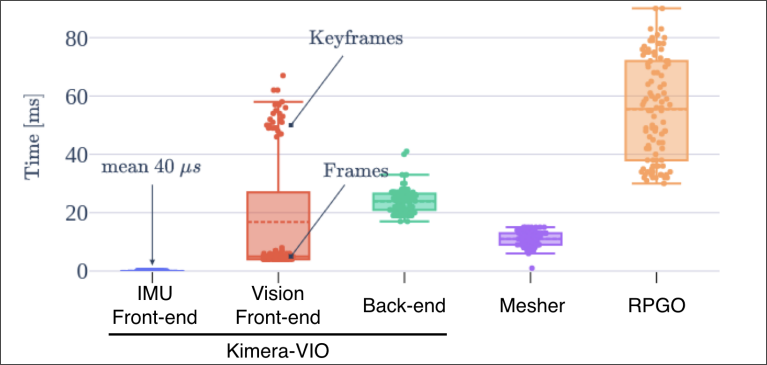
\includegraphics[width=120mm]{Timings}
  \caption{Kimera timings (see \cite{rosinol2020kimera})}\label{Fig:Timings}  
\end{figure}

\section{Conclusion}


{\small                   % use small if you need it
\bibliographystyle{plain}
\bibliography{paper}       % use a bib-file paper.bib to collect your references
}

\end{document}

